\documentclass{article}

%% PAQUETES

% Paquetes generales
\usepackage[margin=2cm, paperwidth=210mm, paperheight=297mm]{geometry}
\usepackage[spanish]{babel}
\usepackage[utf8]{inputenc}
\usepackage{gensymb}

% Paquetes para estilos
\usepackage{textcomp}
\usepackage{setspace}
\usepackage{colortbl}
\usepackage{color}
\usepackage{color}
\usepackage{upquote}
\usepackage{xcolor}
\usepackage{listings}
\usepackage{caption}
\usepackage[T1]{fontenc}
\usepackage[scaled]{beramono}

% Paquetes extras
\usepackage{amssymb}
\usepackage{float}
\usepackage{graphicx}
\usepackage{url}
\usepackage{color}


%% Fin PAQUETES


% Definición de preferencias para la impresión de código fuente.
%% Colores
\definecolor{gray99}{gray}{.99}
\definecolor{gray95}{gray}{.95}
\definecolor{gray75}{gray}{.75}
\definecolor{gray50}{gray}{.50}
\definecolor{gray25}{gray}{.25}
\definecolor{keywords_blue}{rgb}{0.13,0.13,1}
\definecolor{comments_green}{rgb}{0,0.5,0}
\definecolor{strings_red}{rgb}{0.9,0,0}

%% Caja de código
\DeclareCaptionFont{white}{\color{white}}
\DeclareCaptionFont{style_labelfont}{\color{black}\textbf}
\DeclareCaptionFont{style_textfont}{\it\color{black}}
\DeclareCaptionFormat{listing}{\colorbox{gray95}{\parbox{16.78cm}{#1#2#3}}}
\captionsetup[lstlisting]{format=listing,labelfont=style_labelfont,textfont=style_textfont}

\lstset{
	aboveskip = {1.5\baselineskip},
	backgroundcolor = \color{gray99},
	basicstyle = \ttfamily\footnotesize,
	breakatwhitespace = true,   
	breaklines = true,
	captionpos = t,
	columns = fixed,
	commentstyle = \color{comments_green},
	escapeinside = {\%*}{*)}, 
	extendedchars = true,
	frame = lines,
	keywordstyle = \color{keywords_blue}\bfseries,
	language = Oz,                       
	numbers = left,
	numbersep = 5pt,
	numberstyle = \tiny\ttfamily\color{gray50},
	prebreak = \raisebox{0ex}[0ex][0ex]{\ensuremath{\hookleftarrow}},
	rulecolor = \color{gray75},
	showspaces = false,
	showstringspaces = false, 
	showtabs = false,
	stepnumber = 1,
	stringstyle = \color{strings_red},                                    
	tabsize = 2,
	title = \null, % Default value: title=\lstname
	upquote = true,                  
}

%% FIGURAS
\captionsetup[figure]{labelfont=bf,textfont=it}
%% TABLAS
\captionsetup[table]{labelfont=bf,textfont=it}

% COMANDOS

%% Titulo de las cajas de código
\renewcommand{\lstlistingname}{Código}
%% Titulo de las figuras
\renewcommand{\figurename}{Figura}
%% Titulo de las tablas
\renewcommand{\tablename}{Tabla}
%% Referencia a los códigos
\newcommand{\refcode}[1]{\textit{Código \ref{#1}}}
%% Referencia a las imagenes
\newcommand{\refimage}[1]{\textit{Imagen \ref{#1}}}


\begin{document}
\pagenumbering{roman}
\setcounter{page}{5}



% TÍTULO, AUTORES Y FECHA
\begin{titlepage}
	\vspace*{\fill}
	\begin{center}
		\Large 75.42 Taller de Programación I \\
		\Huge TP N°5: Archivos Ubicuos \\
		\bigskip\huge\textit{Grupo 04} \\
		\bigskip\bigskip\bigskip\bigskip\bigskip\bigskip
		\bigskip\bigskip\bigskip\bigskip\bigskip\bigskip\bigskip
		\medskip\huge\textit{``Manual de Usuario''} \\
		\date{}
	\end{center}
	\vspace*{\fill}
\end{titlepage}
\newpage




% ÍNDICE
\tableofcontents
\newpage
\pagenumbering{arabic}




% INSTALACION
\section{Instalación}
	
	Se detalla aquí los pasos a seguir en el proceso de instalación de la aplicación \textit{AU}.
\bigskip



% INSTALACION - Requerimientos de software
\subsection{Requerimientos de software}
	
	Asegúrese de que su sistema cumple los requisitos de software mínimos recomendados, los cuales se encuentran especificados a continuación:
	\medskip

	\begin{itemize}
	\itemsep=5pt \topsep=0pt \partopsep=0pt \parskip=0pt \parsep=0pt

		\item \textit{Sistemas operativos}: GNU/Linux (x86 y x86-64, distribuciones Linux basadas en RPM y DEB);

		\item \textit{Librerias externas}: \begin{enumerate}
							\item gtkmm 3.0
							\item cairomm 1.0
							\item Biblioteca socket.h standard de c++
							\item Biblioteca pthread.h standard de c++
							\end{enumerate}

		\item \textit{Compilador}: g++ (\url{http://gcc.gnu.org/});

		\item \textit{Herramientas}: Make (\url{http://www.gnu.org/software/make/}).

	\end{itemize}
\bigskip



% INSTALACION - Requerimientos de hardware
\subsection{Requerimientos de hardware}
	
	Asegúrese de que su equipo cumple con los requerimientos mínimos de hardware:
	\medskip

	\begin{itemize}
	\itemsep=5pt \topsep=0pt \partopsep=0pt \parskip=0pt \parsep=0pt

		\item \textit{Memoria}: 128MB mínimo, 512MB recomendado;

	\end{itemize}
\bigskip



% INSTALACION - Proceso de Instalación
\subsection{Proceso de Instalación}
	
	Para instalar la aplicación bastará con descomprimir cada
\bigskip




% CONFIGURACION
\section{Configuración}
	
	[ Colocar texto aquí ]
\bigskip




% FORMA DE USO
\section{Forma de uso}
	
	Para ejecutar el programa, se deberá correr por consola \textit{./server} si se quiere iniciar el server, \textit{./monitor} para iniciar la aplicación monitor o \textit{./client} para iniciar la aplicación cliente. También se puede iniciar cada aplicación realizando un doble click sobre los archivos \textit{server}, \textit{monitor} o \textit{client}.

\subsection{Aplicación Servidor}
\smallskip 
	Al ejecutar la aplicacion servidor, se observara una consola como la siguiente, en la que corre la aplicación. Para terminar la ejecución de la aplicación, se deben seguir las instrucciones en pantalla (Presionar la letra 'q').	
	\begin{figure}[h]
       \centering
       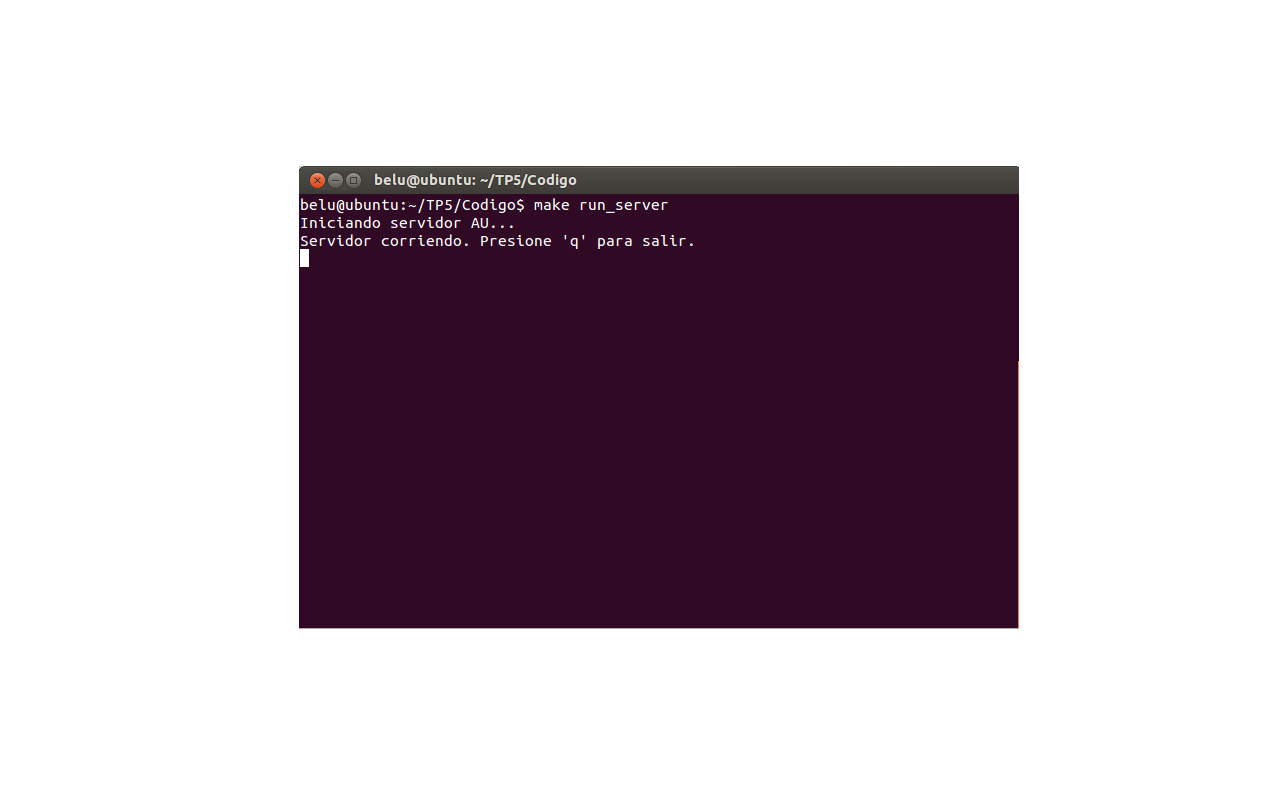
\includegraphics[width=0.85\textwidth]{Server.png}
	\bigskip
       \caption{Consola del server.}
	\end{figure}

\subsection{Aplicación Monitor}
\smallskip
	Al ejecutar la aplicación monitor, se observa una pantalla de inicio de sesión en la que se debe ingresar el nombre ADMMONITOR y la clave 'admin1234'. Alli, se inicia la comunicación entre el servidor (que debe estar corriendo) y el monitor.
	\begin{figure}[h]
       \centering
       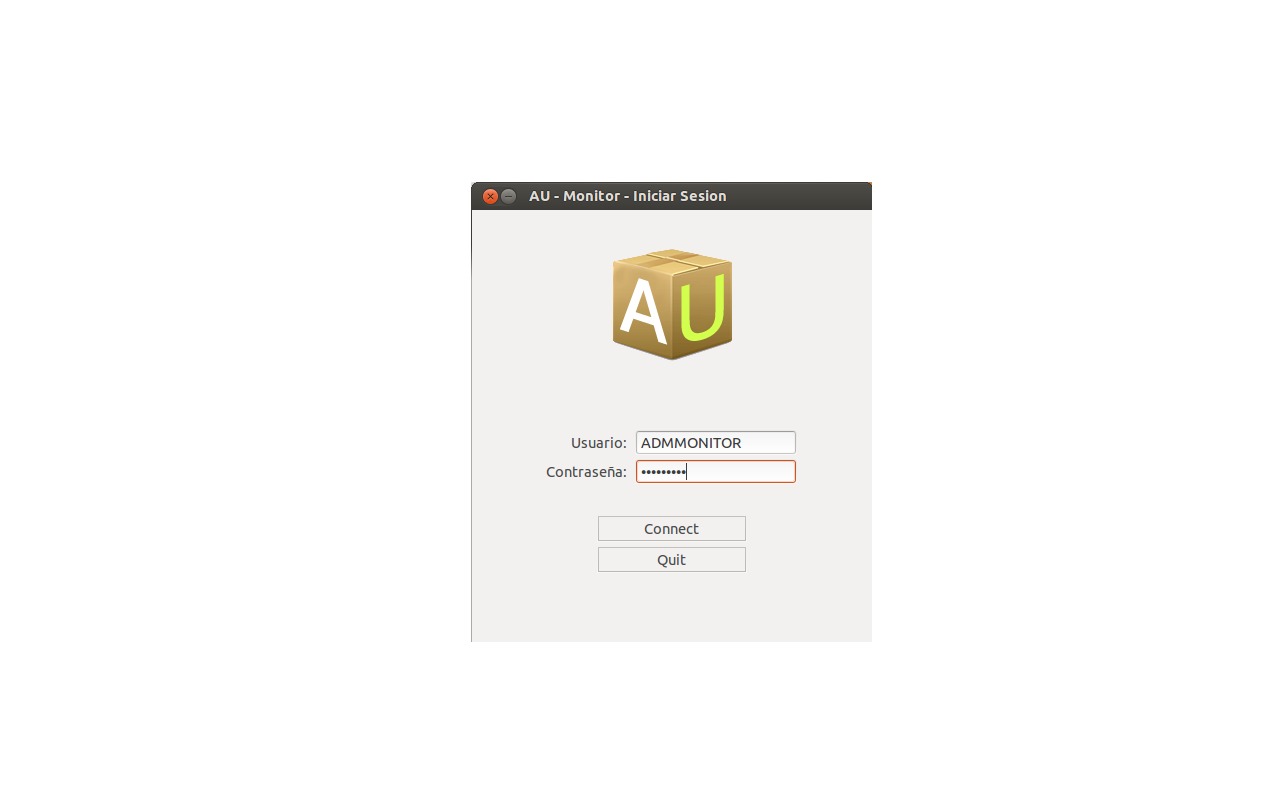
\includegraphics[width=0.85\textwidth]{InicioMonitor.png}
	\bigskip
       \caption{Inicio de sesion del monitor.}
	\end{figure}
	Luego de iniciar sesión correctamente, se accede a una pantalla como la siguiente, donde se pueden observar los siguientes menu de opciones: 
	\begin{figure}[h]
       \centering
       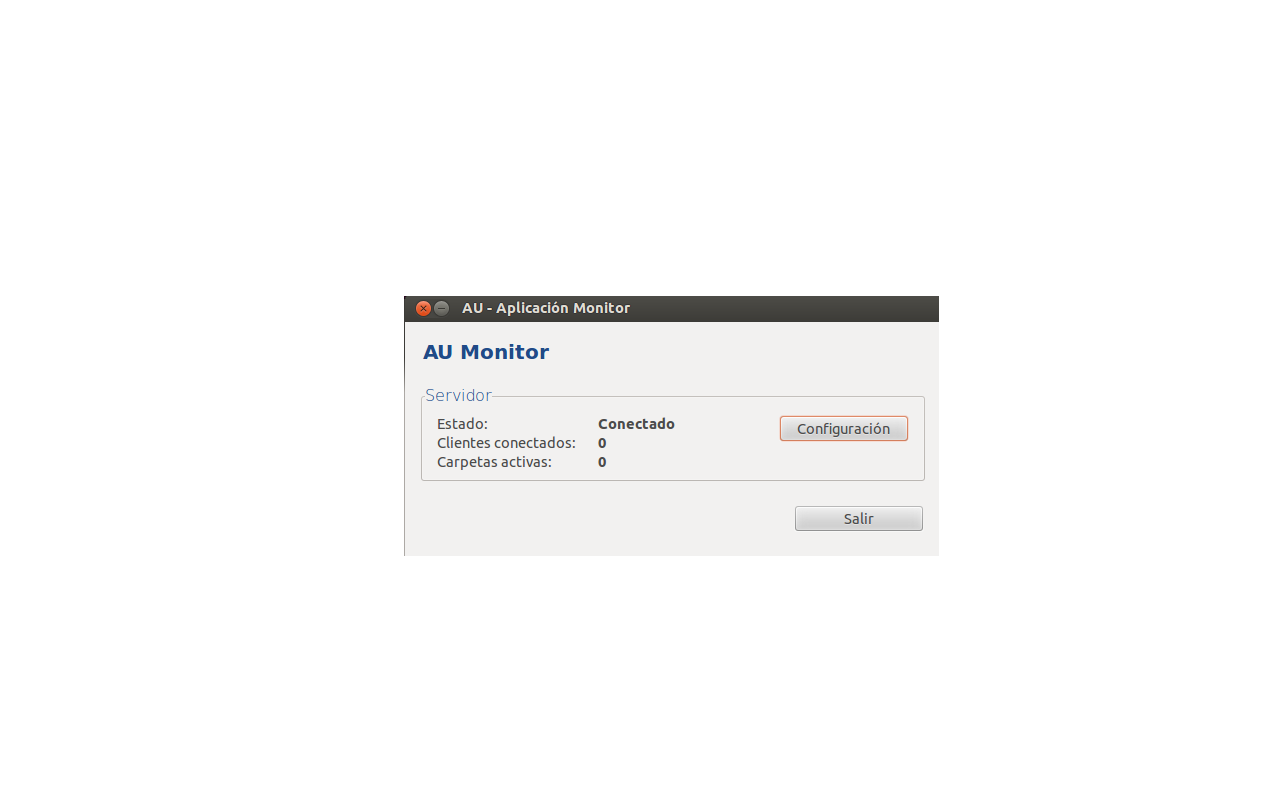
\includegraphics[width=0.85\textwidth]{MonitorPPal.png}
	\bigskip
       \caption{Vista inicial del monitor.}
	\end{figure}
	Desde la opción \textit{Administrar Usuarios}, se pueden administrar las cuentas de todos los usuarios registrados o por registar. Se pueden ingresar nuevos clientes, utilizando el boton \textit{Agregar Usuario}. De aquí, se pasa a una ventana en donde se debe ingresar 'Nombre de usuario' y 'Contraseña'. Para guardar los cambios, presionar 'Guardar'.
	\begin{figure}[h]
       \centering
       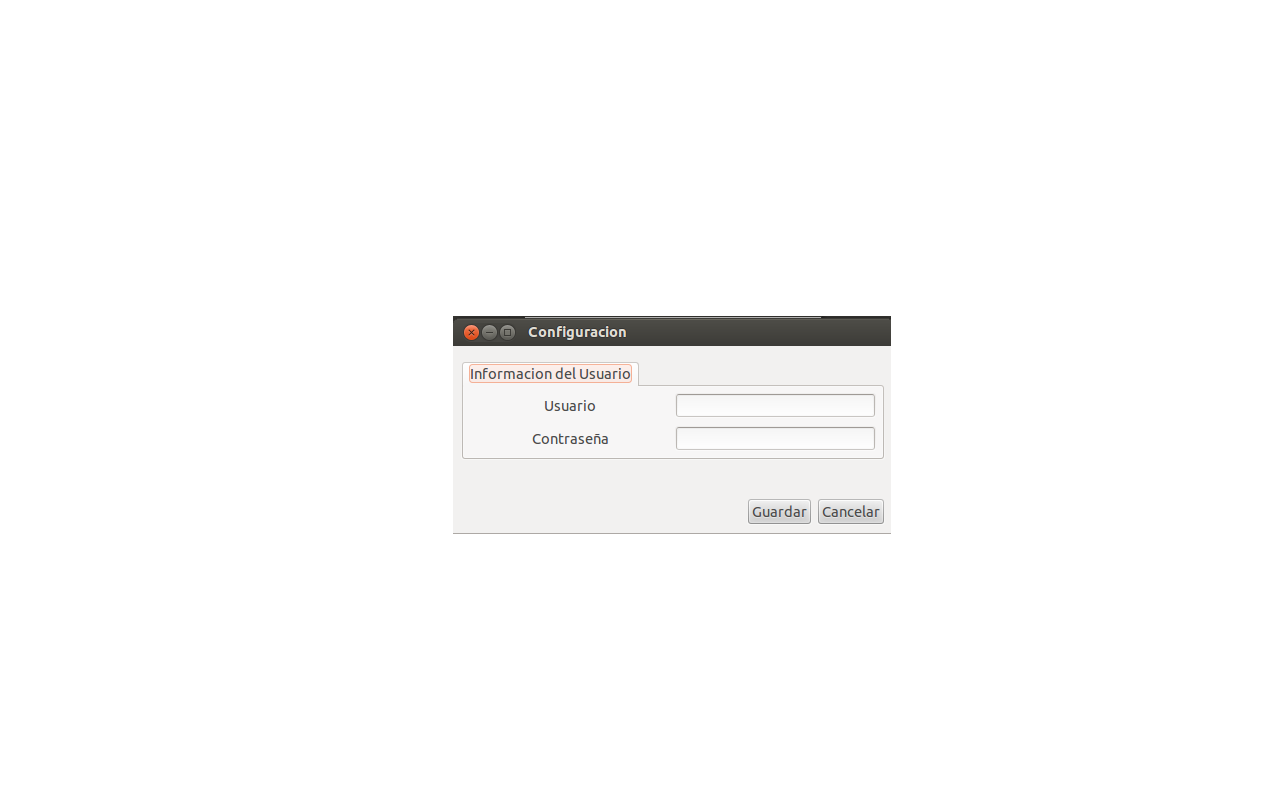
\includegraphics[width=0.85\textwidth]{NuevoUsuario.png}
	\bigskip
       \caption{Interfaz de nuevo usuario.}
	\end{figure}
	Para modificar usuarios existentes, se debe seleccionar uno de la lista y presionar el boton \textit{Modificar Usuario}. Solamente se podrá modificar la clave asociada al usuario que se seleccionó.
	\begin{figure}[h]
       \centering
       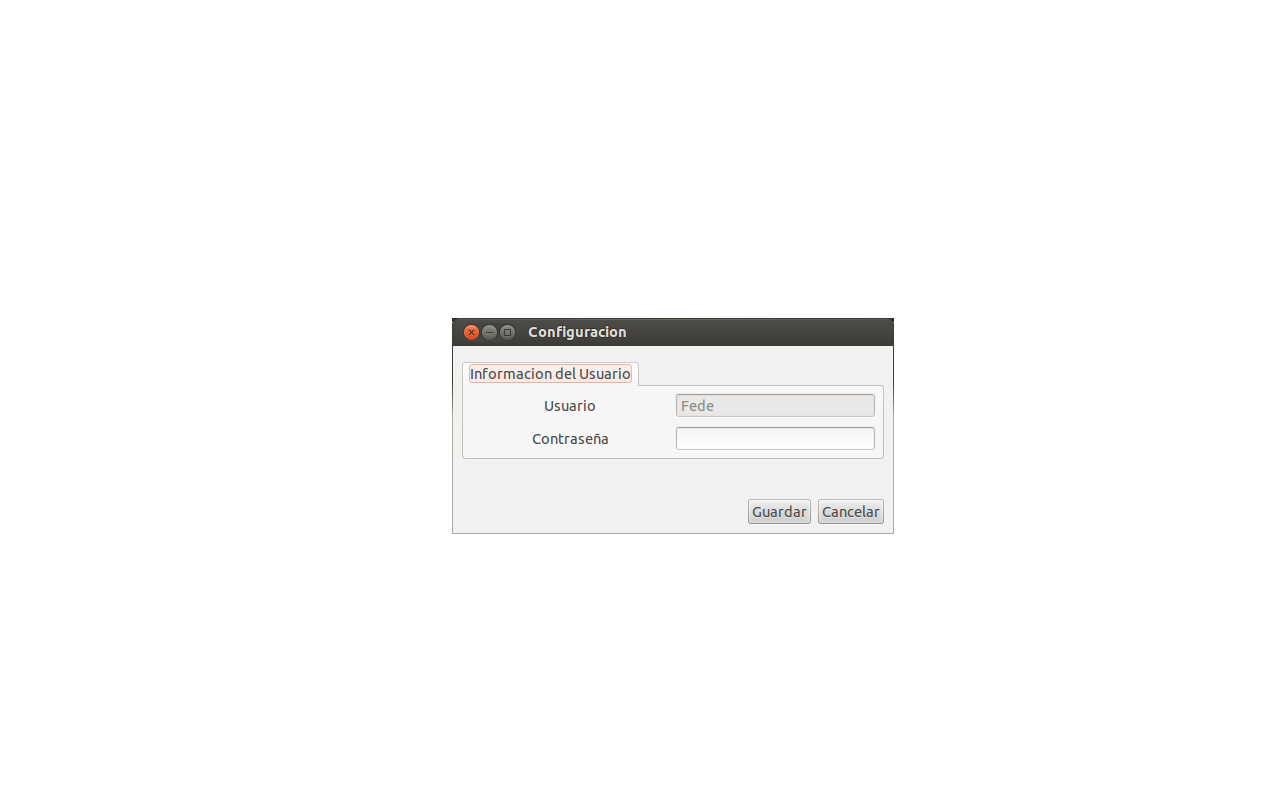
\includegraphics[width=0.85\textwidth]{ModifUsuario.png}
	\bigskip
       \caption{Interfaz de modificar usuario.}
	\end{figure}
	Luego, se podrá eliminar un usuario existente, seleccionandolo de la lista y presionando el boton \textit{Eliminar Usuario}. Se abre una ventana preguntando si realmente desea eliminarlo.
	\begin{figure}[h]
       \centering
       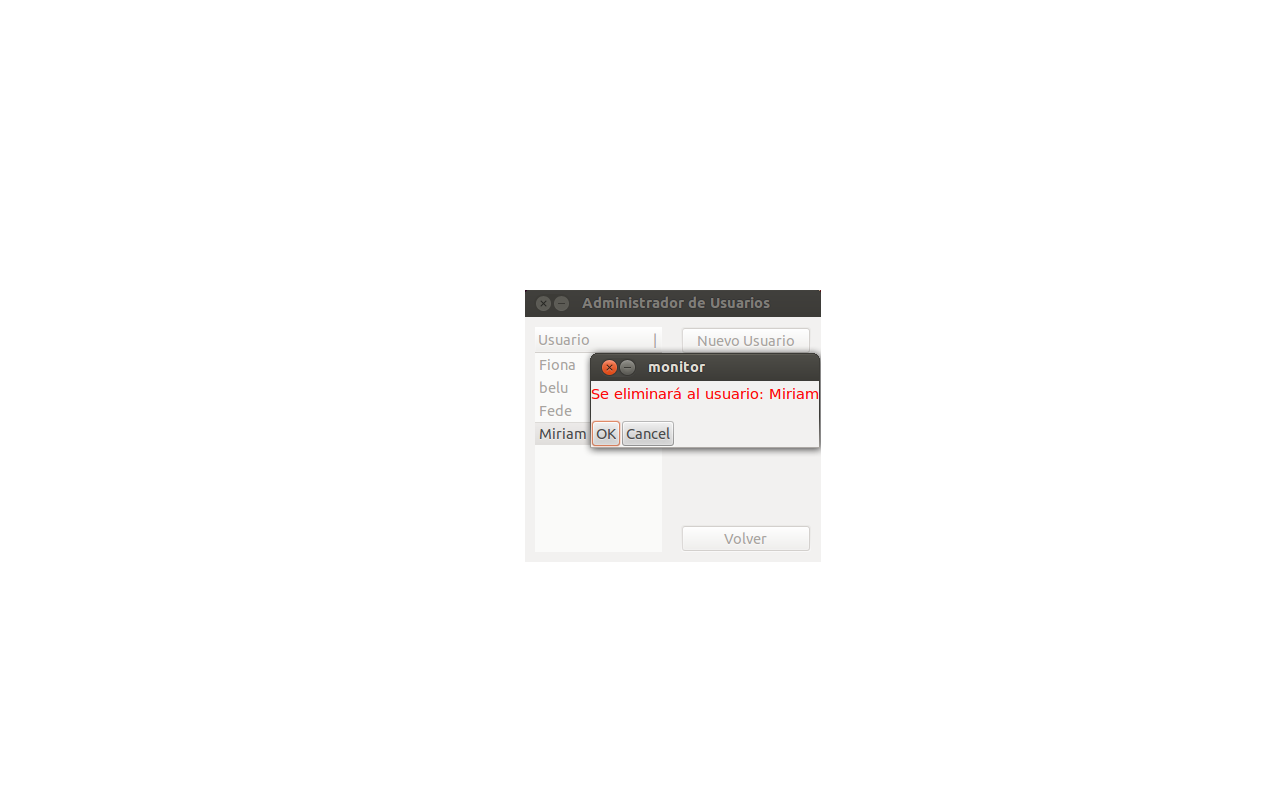
\includegraphics[width=0.85\textwidth]{EliminarUsuario.png}
	\bigskip
       \caption{Eliminar Usuario.}
	\end{figure}

\subsection{Aplicación Cliente}
\smallskip
	Al ejecutar la aplicación cliente, se observara una pantalla de inicio de sesión en la que se debe ingresar el nombre de usuario y contraseña. 
	\begin{figure}[h]
       \centering
       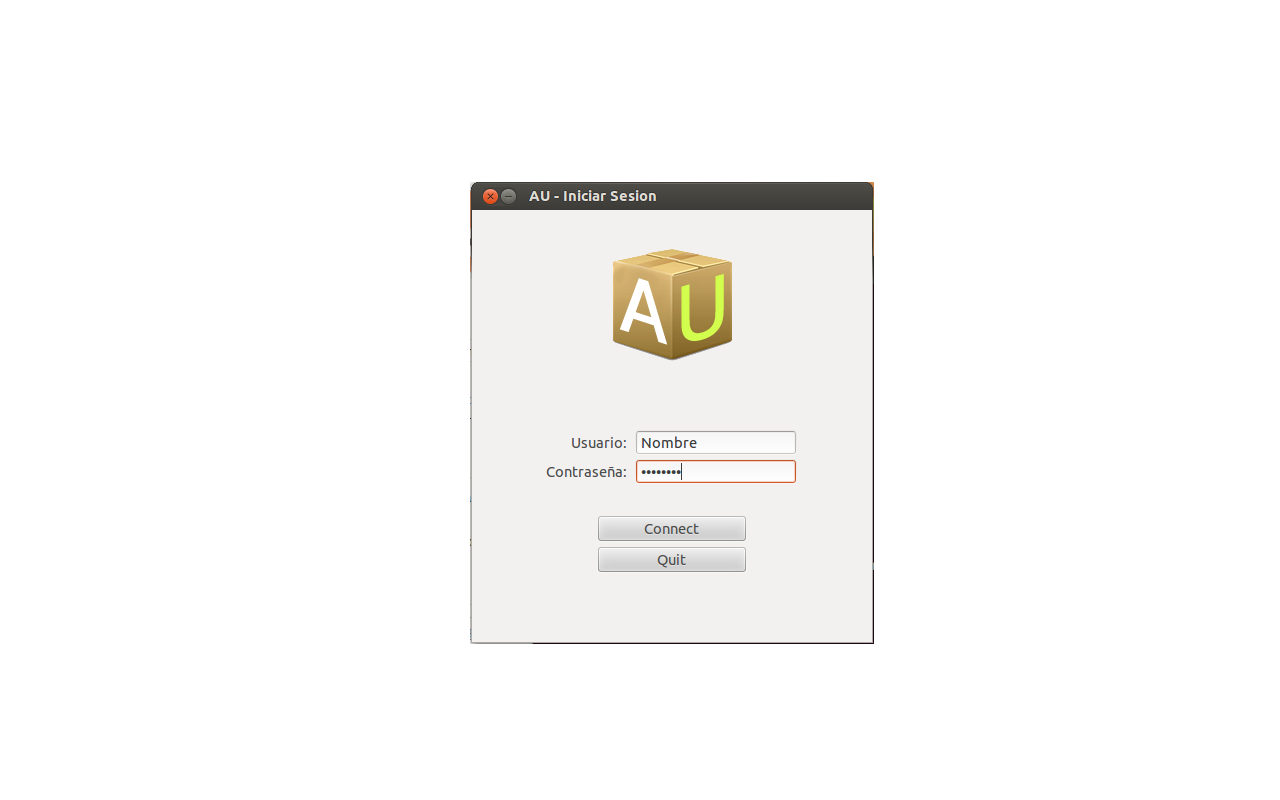
\includegraphics[width=0.85\textwidth]{InicioSesionCli.png}
	\bigskip
       \caption{Inicio de sesion de cliente.}
	\end{figure}
	Luego, al entrar en el proceso de sincronización, se puede ver la pantalla de esta forma:
	\begin{figure}[h]
       \centering
       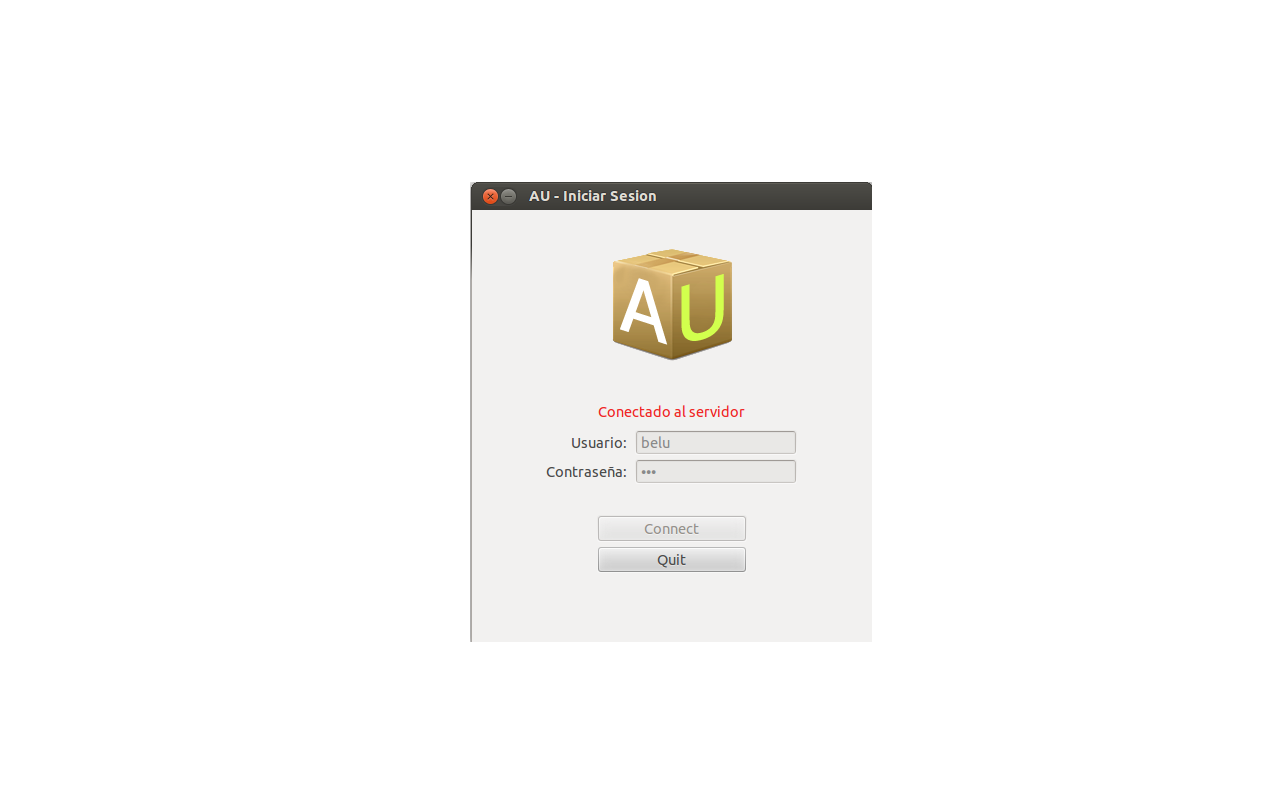
\includegraphics[width=0.85\textwidth]{Sincronizando.png}
	\bigskip
       \caption{Sincronizacion.}
	\end{figure}
\bigskip




% APENDICE DE ERRORES
\section{Apéndice de errores}
	
	[ Colocar texto aquí ]
\bigskip



\end{document}
